\chapter{Realisierung des Systems}
Zu Beginn der Realisierung erfolgt die Anordnung aller benötigten Buchstaben für die verschiedenen Funktionen und Wortdarstellungen. 
Ziel ist die Umsetzung eines möglichst kompakten und quadratischen Rasters.
Die erste Konzeptentwicklung erfolgt auf einem Tablet. 
Dabei werden die Positionen der einzelnen Buchstaben sowie deren Zuordnung zu den jeweiligen Funktionen skizziert. 
Diese Vorgehensweise ermöglicht eine flexible Anpassung des Layouts, da die Buchstaben und Symbole noch verschoben und umpositioniert werden können.
Das Ergebnis der Konzeptentwicklung ist in Abb.~\ref{fig:Konzeptentwicklung} dargestellt.

\begin{figure}[H]
	\centering
	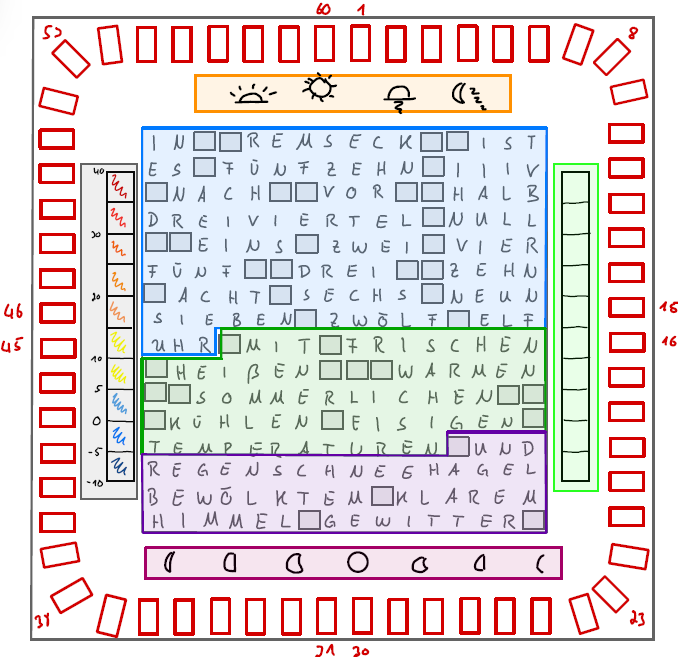
\includegraphics[width=0.7\linewidth]{inhalt/bilder/ErstesKonzept.png}
	\caption[Erster Konzeptentwurf der WordClock]{Erster Konzeptentwurf, der als Grundlage für das Design verwendet wird. Im blau markierten Bereich wird die Uhrzeit in Stunden und Minuten angezeigt. Im grün markierten Bereich werden im Textfeld die Außentemperatur sowie rechts daneben die Raumfeuchtigkeit in Form einer Skala dargestellt. Im lila markierten Bereich wird im Textfeld die aktuelle Wetterlage angezeigt. Im magenta markierten Bereich unterhalb des Textfeldes wird die aktuelle Mondphase dargestellt. Im grau markierten Bereich links vom Textfeld wird die Innenraumtemperatur als Skala angezeigt. Im orange markierten Bereich oberhalb des Textfeldes wird die aktuelle Tageszeit dargestellt. Abschließend werden die Sekunden als Lauflicht in den roten Kästchen am Rand der WordClock angezeigt.}
	\label{fig:Konzeptentwicklung}
\end{figure}

Weiterhin soll die WordClock über einen sogenannten Boot-Modus verfügen, während sie startet. 
Dieser Ablauf ist ebenfalls in der Konzeptionierungsphase entstanden und in Abb.~\ref{fig:Konzeptentwicklung_boot} dargestellt.

\begin{figure}[H]
    \centering
    \begin{subfigure}[t]{0.4\textwidth}
        \centering
        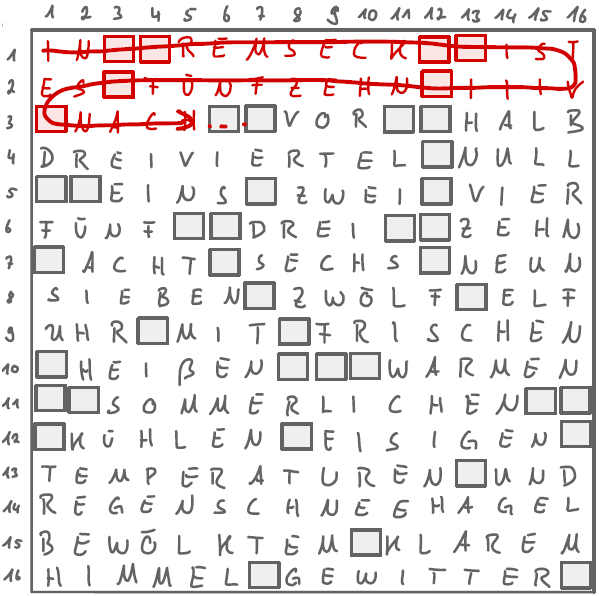
\includegraphics[width=\linewidth]{inhalt/bilder/ErstesKonzept_bootA.png}
        \caption{Startend von 1-1 alle LEDs der Reihe nach an in Schlangenlinien.}
        \label{fig:Konzeptentwicklung_bootA}
    \end{subfigure}
    \hfill
    \begin{subfigure}[t]{0.4\textwidth}
        \centering
        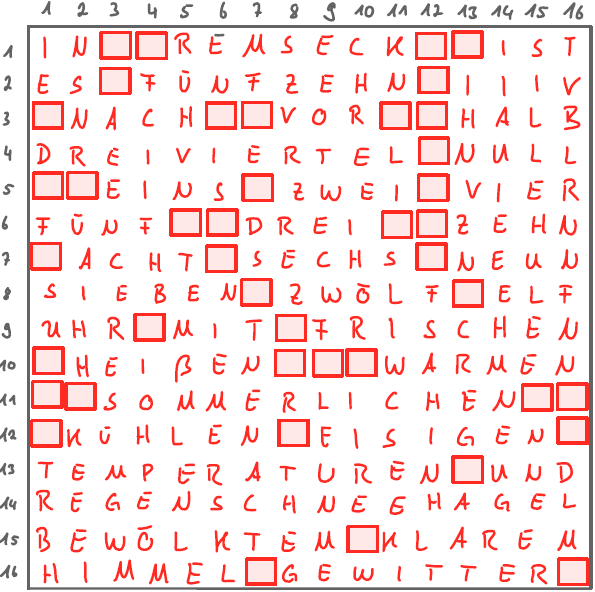
\includegraphics[width=\linewidth]{inhalt/bilder/ErstesKonzept_bootB.png}
        \caption{Alle LEDs sind kurz an.}
        \label{fig:Konzeptentwicklung_bootB}
    \end{subfigure}
    \vspace{0.8em}
    \begin{subfigure}[t]{0.4\textwidth}
        \centering
        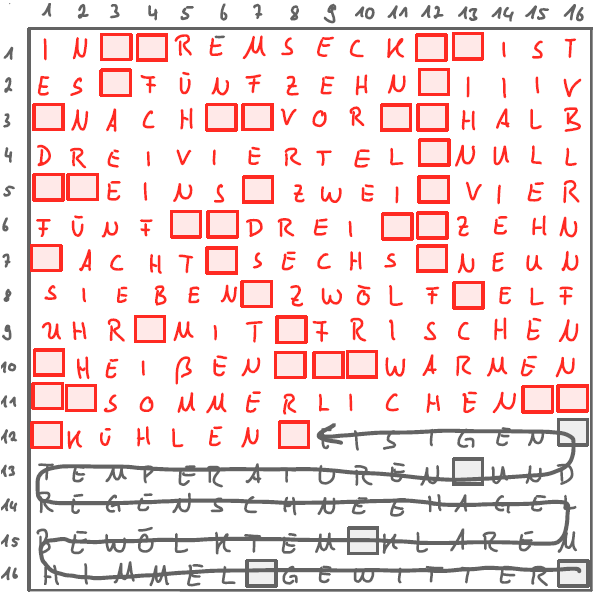
\includegraphics[width=\linewidth]{inhalt/bilder/ErstesKonzept_bootC.png}
        \caption{Startend von 16-16 gehen alle LEDs entgegengesetzt wieder aus.}
        \label{fig:Konzeptentwicklung_bootC}
    \end{subfigure}
    \hfill
    \begin{subfigure}[t]{0.4\textwidth}
        \centering
        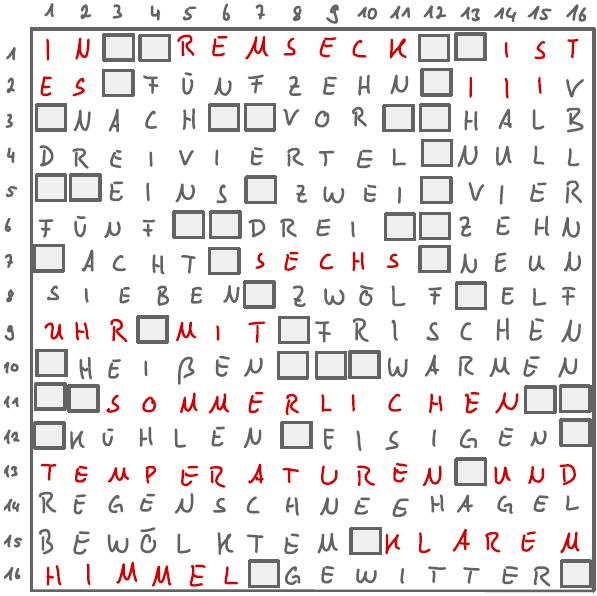
\includegraphics[width=\linewidth]{inhalt/bilder/ErstesKonzept_bootD.png}
        \caption{Alle LEDs sind kurz aus. Wenn die WordClock alles fertig geladen hat, geht diese in den Anzeigemodus, ansonsten beginnt der Ablauf von vorne.}
        \label{fig:Konzeptentwicklung_bootD}
    \end{subfigure}
    \caption[Ablauf des Boot-Modus]{Ablauf des Boot-Modus der WordClock um anzuzeigen, dass diese gerade startet und die Werte abgerufen und initialisiert werden.}
    \label{fig:Konzeptentwicklung_boot}
\end{figure}

Zur Bestimmung der minimal nötigen Buchstabengröße wird ein empirischer Ansatz gewählt. 
Hierfür werden Testdrucke mit unterschiedlichen Schriftgrößen erstellt.
Das entscheidende Kriterium ist die gute Lesbarkeit aus einer Entfernung von etwa 5 m. 
Auf Basis der ermittelten Schriftgröße ergibt sich die Gesamtgröße der WordClock.
Weiterhin kann damit der Abstand ermittelt und leicht angepasst werden, den die \gls{led}s voneinander haben müssen, damit eine \gls{led} pro Buchstabe platziert wird.
Damit kann das passende \gls{led}-Band gewählt werden, auf welchem die \gls{ws2812b}-\gls{led}s integriert sind.
So muss nicht jede \gls{led} einzeln verlötet werden.  
Zuletzt bildet dies die Grundlage für die Aufteilung der Bauteile im Hinblick auf den Fertigungsprozess. 
Da das verfügbare Druckbett des verfügbaren \gls{3ddrucker} auf ein Volumen von 250 mm × 250 mm × 250 mm begrenzt ist, erfolgt eine entsprechende Segmentierung der Konstruktion und die Frontplattenbauteile können konstruiert werden.